El objetivo es encontrar la dinámica de la formación de los fragmentos para sistemas que se expanden de acuerdo al modelo del pequeño \emph{big bang}.
Esta expansión se parece a la evolución de las colisiones de estrellas de neutrones.
A partir de una configuración de equilibrio, expandimos el sistema homogéneamente hasta llegar a una configuración asintótica (i.\ e.\ densidades muy bajas).
Estudiamos, con cuatro algoritmos reconocedores de fragmentos distintos, la distribución de fragmentos a lo largo de esta expansión y la dinámica de la formación de fragmentos.

Estudiando la topología de los estados de equilibrio, antes de la expansión, reprodujimos las pastas usuales y, además, una nueva fase que hemos llamado \emph{pregnocchi}, que consiste de agregados de protones embebidos en un  \emph{mar de neutrones}.
Identificamos distintos regímenes de fragmentación, dependiendo de la temperatura inicial y la velocidad de expansión.
En particular, para los ya mencionados \emph{pregnocchi}, una nube de neutrones rodea a los fragmentos a lo largo de los comienzos de la expansión, resultando en sistemas con configuraciones compatibles con la emergencia del \emph{r-proccess}.

Mostramos que una identificación adecuada de la distribución de fragmentos depende del algoritmo de reconocimiento de fragmentose scogido, y que el Algoritmo de Reconocimiento Temprano de Fragmentos (ECRA) fue el más estable.
Este enfoque nos permitió identificar la dinámica de la formación de fragmentos.
Estos cálculos pueden ser el comienzo de una comparación entre los experimentos de fragmentación terrestres y los estudios de estrellas de neutrones.
\section{Dependencia de la configuración con el potencial}

\begin{figure*}
  \begin{subfigure}{.3\linewidth}
    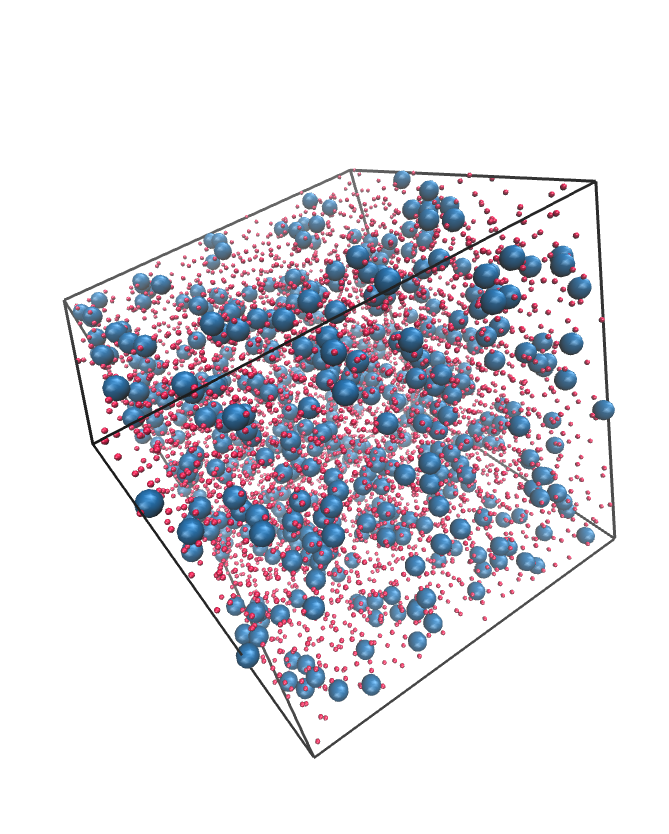
\includegraphics[width=\columnwidth]{dinamica/pregnocchi_med.png}
    \caption{CMD medium}
  \end{subfigure}
  \begin{subfigure}{.3\linewidth}
    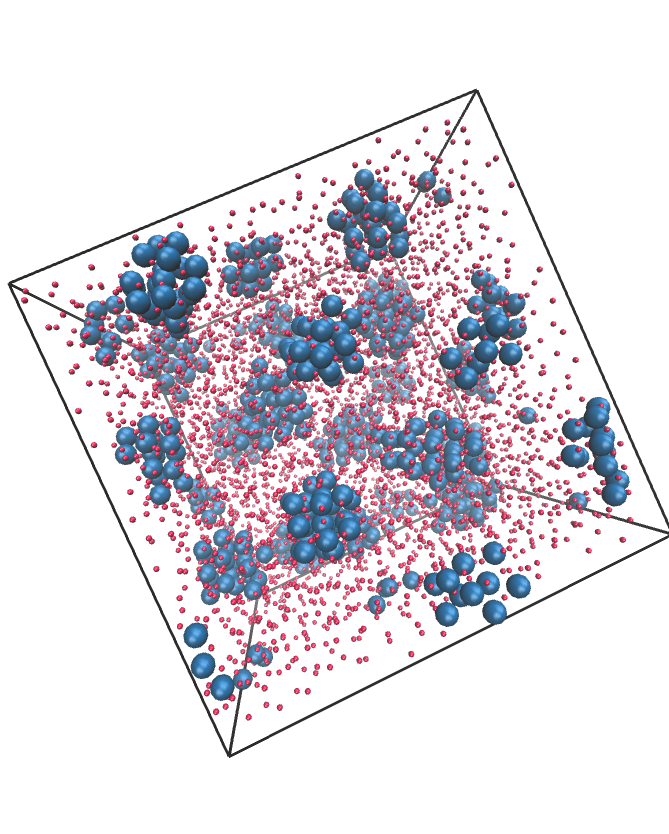
\includegraphics[width=\columnwidth]{dinamica/pregnocchi_newmed.png}
    \caption{New medium}
  \end{subfigure}
  \begin{subfigure}{.3\linewidth}
    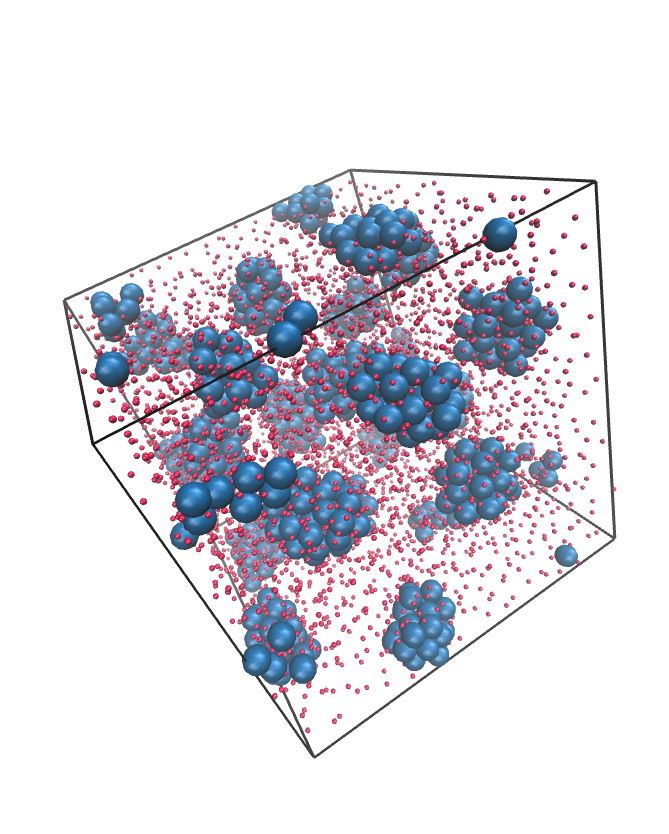
\includegraphics[width=\columnwidth]{dinamica/pregnocchi_horo.png}
    \caption{SSP}
  \end{subfigure}
  \caption{Imágenes de configuraciones para distintas parametrizaciones de la interacción nuclear, todas con las mismas condiciones termodinámicas: $x = 0.1$, $\rho = 0.05\,\text{fm}^{-3}$ y $T = 0.1\,\text{MeV}$.
    Las diferencias cualitativas entre el potencial tipo medio de CMD y las otras dos paramtrizaciones (New Medium y SSP) son evidentes.
    Llamamos estas estructuras que aparecen en New Medium y SSP \emph{pregnocchi}.
    Para facilitar la identificación de la estructura de protones, los neutrones están representados por puntos muy pequeños comparados con los protones.}
\label{fig:x01_potentials}
\end{figure*}

\begin{figure*}
  \begin{subfigure}{.3\linewidth}
    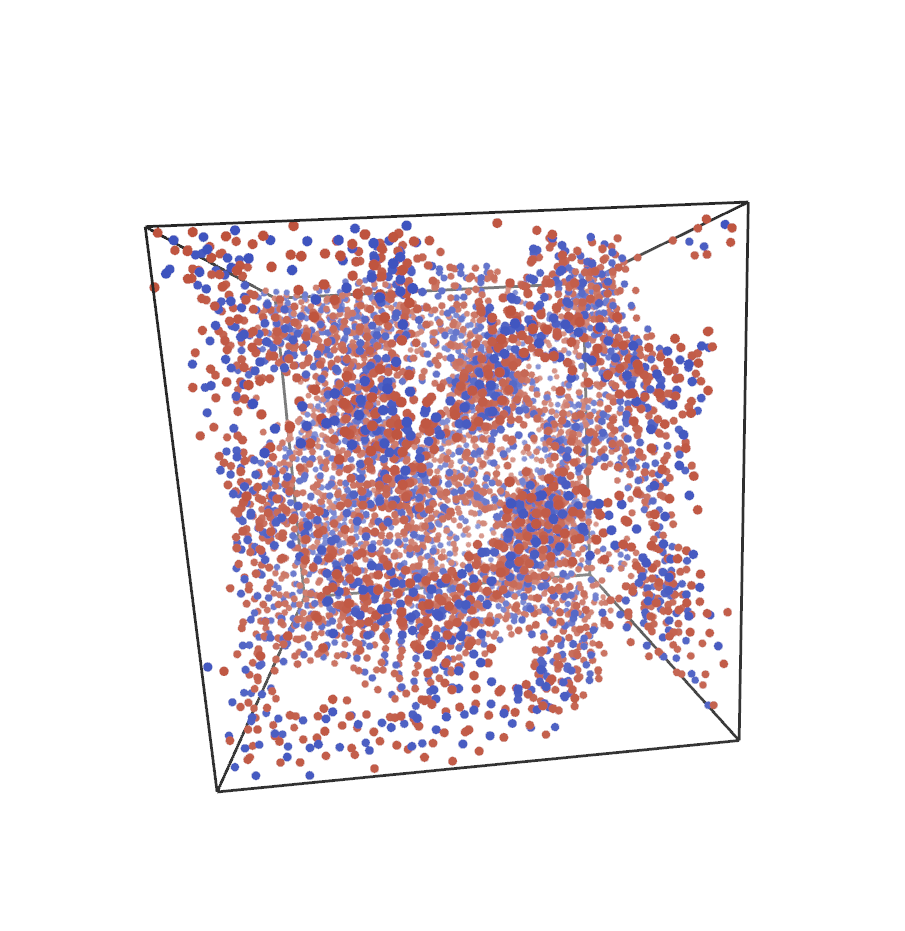
\includegraphics[width=\columnwidth]{dinamica/jungle_gym.png}
    \caption{Medium}
  \end{subfigure}
  \begin{subfigure}{.3\linewidth}
    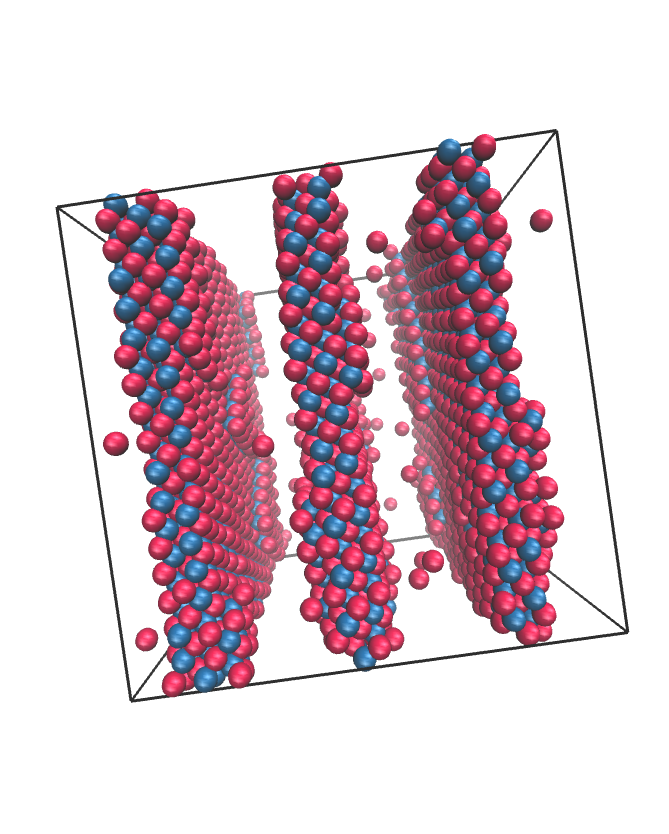
\includegraphics[width=\columnwidth]{dinamica/lasagna_newmed.png}
    \caption{New medium}
  \end{subfigure}
  \begin{subfigure}{.3\linewidth}
    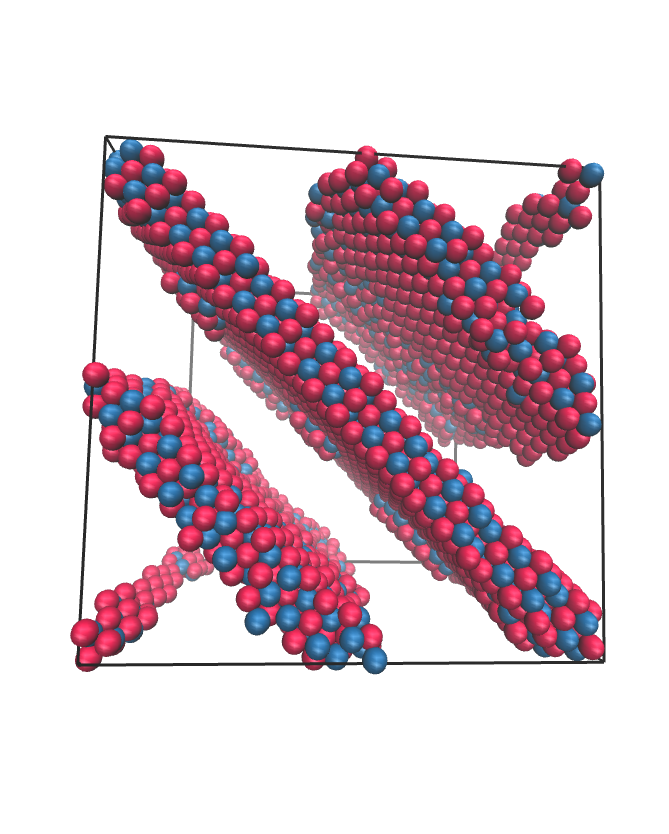
\includegraphics[width=\columnwidth]{dinamica/lasagna_horo.png}
    \caption{SSP}
  \end{subfigure}
  \caption{Imágenes de configuraciones para distintas parametrizaciones de la interacción nuclear, todas con las mismas condiciones termodinámicas: $x = 0.4$, $\rho = 0.05\,\text{fm}^{-3}$ y $T = 0.1\,\text{MeV}$.
    Las diferencias cualitativas entre el potencial tipo medio de CMD y las otras dos paramtrizaciones (New Medium y SSP) son evidentes.
    Mientras que el potencial CMD muestra una estructura de tipo \emph{jungle gym}, tanto New Medium como SSP muestra \emph{lasagna} que son ligeramente diferentes entre sí.}
\label{fig:x04_potentials}
\end{figure*}

Distintos modelos de interacción resultan en distintas ecuaciones de estado y, en consecuencia, distintas configuraciones.
Para comarar, mostramos en la figura~\ref{fig:x01_potentials} distintas imágenes para los tres modelos estudiados: \emph{CMD medium}, \emph{New medium} y \emph{SSP}.
Estas estructuras son cercanas al estado fundamental, con temperatura muy baja ($T = 0.1\,\text{MeV}$), densidad $\rho = 0.05\,\text{fm}^{-3}$ y una fracción de protones de $x = 0.1$.
Las diferencias son notorias: mientras que el potencial \emph{CMD medium} no tienen ninguna estructura identificable, \emph{New medium} y \emph{SSP} muestran claramenta aglomeraciones de protones (debido a la interacción atractiva que median los neutrones) embebidos en un \emph{mar de neutrones}.
Esta estructura la llamaremos \emph{pre-gnocchi}.
Esta es la primera vez que se observa este tipo de estructuras, y es también una muy interesante diferencia \emph{cualitativa} observadas entre parametrizaciones de la ecuación de estado.

Para comparar los potenciales en otra configuración, mostramos en la figura~\ref{fig:x04_potentials} distintas imágenes para los tres modelos que estudiamos: \emph{CMD medium}, \emph{New medium} y \emph{SSP}.
Estas estructuras son cercanas al estado fundamental, con temperatura muy baja ($T = 0.1\,\text{MeV}$), densidad $\rho = 0.05\,\text{fm}^{-3}$ y una fracción de protones de $x = 0.4$.

\section{Distribución Asintótica de Masas}
Cuando el sistema se expande, la estructura se parte en fragmentos finitos
Para tiempos suficientemente largos, estos fragmentos permanecen estables, ya que no interactúan entre sí.
Llamaremos a estos ``fragmentos asintóticos''.

Expandimos distintas configuraciones iniciales con el modelo \emph{New medium} para encontrar la distribución asintótica de masas.
Como primer ejemplo, mostramos en la figura~\ref{fig:asymp_preg} la distribucióñ asintótica de masas (calculada con el algoritmo MSTE) para $x = 0.1$, $\rho = 0.05\,\text{fm}^{-3}$ y $T = 0.8\,\text{MeV}$ para dos velocidades de expansión: \emph{rápida} ($\dot{\eta} = 0.01\,\text{c/fm}$)y \emph{lenta} ($\dot{\eta} = 0.0001\,\text{c/fm}$)
Podemos ver aquí que la expansión lenta permite la existencia de fragmentos con masa de hasta 60 (20 de los cuales son protones) mientras que la expansión rápida produce fragmentos más pequeños de hasta 20 (6 protones).
Este comportamiento es esperado, ya que cuanto más rápida la expansión, mayor la energía de excitación que se le agrega al sistema.
En consecuencia, una expansión más rápida debería romper fragmentos que, de otro modo, serían estables.
Un comportamiento similar se puede ver en la figura~\ref{fig:asymp_las}, donde expandimos el sistema para $x = 0.4$, $\rho = 0.05\,\text{fm}^{-3}$ y $T = 0.1\,\text{MeV}$ para las mismas velocidades de expansión rápida y lenta.
Otra característica relevante de la distribución asintótica de masas (que no se muestra en la figura debido a limitaciones de escala) es que la expansión rápida tiene una fracción no despreciable de neutrones sueltos (cerca del $4\%$) mientras que la expansión lenta presenta muy pocos ($0.1\%$).

\begin{figure}[h]
  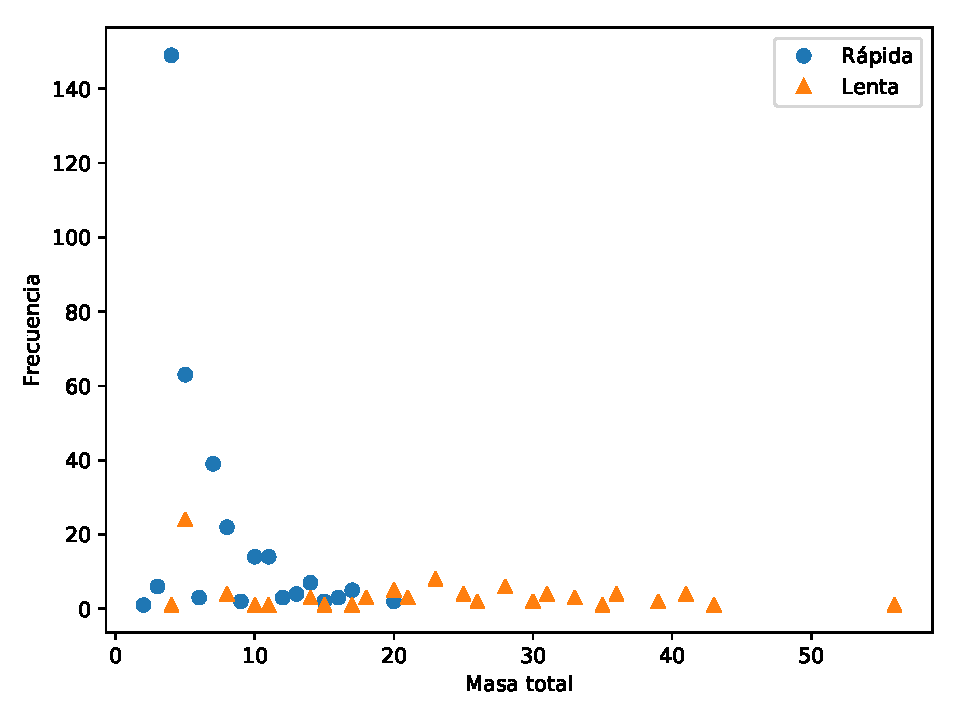
\includegraphics[width=0.8\columnwidth]{dinamica/pregnocchi}
  \caption{Distribución asintótica de masas para $x = 0.1$, $\rho = 0.05\,\text{fm}^{-3}$ y $T = 0.8\,\text{MeV}$ y dos velocidades de expansión distintas: \emph{rápida} $\dot{\eta} = 0.01\,\text{c/fm}$ y \emph{lenta} $\dot{\eta} = 0.0001\,\text{c/fm}$.}
\label{fig:asymp_preg}
\end{figure}

\begin{figure}[h]
  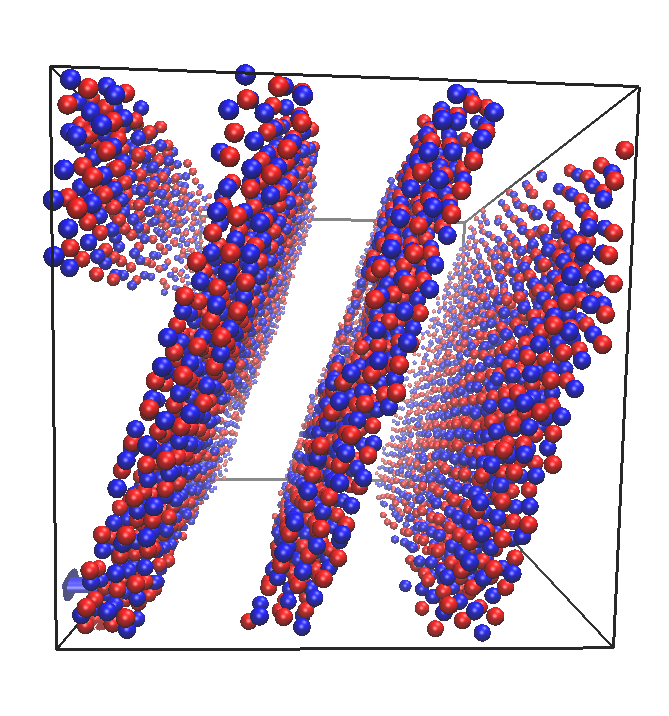
\includegraphics[width=0.8\columnwidth]{dinamica/lasagna}
  \caption{Distribución asintótica de masas para $x = 0.4$, $\rho = 0.05\,\text{fm}^{-3}$ y $T = 0.1\,\text{MeV}$ y dos velocidades de expansión distintas: \emph{rápida} $\dot{\eta} = 0.01\,\text{c/fm}$ y \emph{lenta} $\dot{\eta} = 0.0001\,\text{c/fm}$.}
\label{fig:asymp_las}
\end{figure}


\section{Formación de fragmentos}
\newcommand{\tabfig}[1]{\includegraphics[width=0.25\linewidth]{dinamica/#1}}

\begin{table*}
  \centering
  \begin{tabular}{cccc}
    \toprule
    & Lasagna (expansión rápida) & Lasagna (expansión lenta) & Pregnocchi \\
    \midrule
    $\rho = 0.05\,\text{fm}^{-3}$ & \tabfig{las_fast_0} & \tabfig{las_slow_0} & \tabfig{pregnocchi_0} \\
    $\rho = 0.0001\,\text{fm}^{-3}$ & \tabfig{las_fast_100} & \tabfig{las_slow_100} & \tabfig{pregnocchi_100} \\
    $\rho = 0.00003\,\text{fm}^{-3}$ & \tabfig{las_fast_400} & \tabfig{las_slow_400} & \tabfig{pregnocchi_400} \\
    \bottomrule
  \end{tabular}
  \caption{Tres distintas expansiones de materia de estrellas de neutrones: Lasagna (expansión rápida): $x = 0.4$, $\dot{\eta} = 0.01\text{c/fm}$, $T = 0.8\,\text{MeV}$;
    Lasagna (expansión lenta): $x = 0.4$, $\dot{\eta} = 0.0001\text{c/fm}$, $T = 0.8\,\text{MeV}$;
    Pregnocchi: $x = 0.1$, $\dot{\eta} = 0.0001\text{c/fm}$, $T = 0.1\,\text{MeV}$}
\label{tbl:expansion}
\end{table*}

Ahora nos centramos en el análisis de algunos ejemplos de la evolución del sistema en el tiempo: cuándo y cómo se forman los fragmentos asintóticos.
Tomaemos primero la expansión del sistema con $x = 0.4$, $\rho = 0.05\,\text{fm}^{-3}$ y $T = 0.5\,\text{MeV}$.
Mostramos en las primeras dos columnas de la tabla~\ref{tbl:expansion} los estados iniciales y asintótico con la expansión rápida y lenta para la \emph{lasagna}.
Mientras que la condición inicial es un cluster infinito, en el régimen asintótico tenemos una distribución de fragmentos con muchos fragmentos finitos.
Es intereasnte notar que la expansión rápida se parece a una fractura mecánica, en la que los fragemtnos se forman dentro de cada hoja de la \emph{lasagna}, mientras que la expansión lenta parece más una expansión térmica en la que el sistema asintótico pierde todo tipo de similaridad con la estructura original.
Los fragmentos se parten en muchos porque su tamaño tan grande no puede soportar la energía asociada con la expansión del sistema.

Un escenario muy interesante es la expansión del sistema con baja fracción de protones: $x = 0.1$, $\rho = 0.05\,\text{fm}^{-3}$ y $T = 0.1\,\text{MeV}$.
En la tercera columna de la tabla~\ref{tbl:expansion} mostramos tanto la condición inicial como la configuración asintótica para $\dot{\eta} = 0.0001\,\text{c/fm}$.

A diferencia del escenario anterior, aquí hay una clara estructura de protones: los fragmentos existen desde el comienzo, immersos en un mar de neutrones.
Pueden ser identificados visualmente si dibujamos los protones con un tamaño mucho mayor que el de los neutrones, como se ve en este conjunto de figuras.
A medida que el sistema se expande, se modifica.
Esto genera la siguiente pregunta: ¿la distribución de fragmentos se modifica sustancialmente?
La respuesta a esta pregunta requiere de un análisis profundo de la evolución temporal de la distribucióñ de fragmentos, y no podemos confiar en una inspección visual; necesitamos usar algoritmos de reconocimiento de fragmentos.
Este tipo de análisis ha sido realizado previamente para sistemas finitos, por ejemplo en Ref.~\cite{dorso_fluctuation_1994, strachan_fragment_1997}.
En la figura~\ref{fig:mste_pregnocchi} mostramos las configuraciones iniciales y final con el algoritmo de MSTE.\@
Podemos notar que la distribución de clusters cambia radicalmente en ambos aspectos: el tamaño y la fracción de protones.
El cambio en la fracción de protones es de esperar ya que, a medida que el sistema se expande, menos neutrones están en el rango del fragmento de protones.
Sin emgargo, este efecto solo no explica el cambio de tamaño: mientras que la condición inicial muestra un fragmento de hasta 80 protones, el fragmento más grande de la distribución asintótica tiene aproximadamente 30 protones.
¿Se rompió un cluster mientras el sistema se expandía?

\begin{figure}
  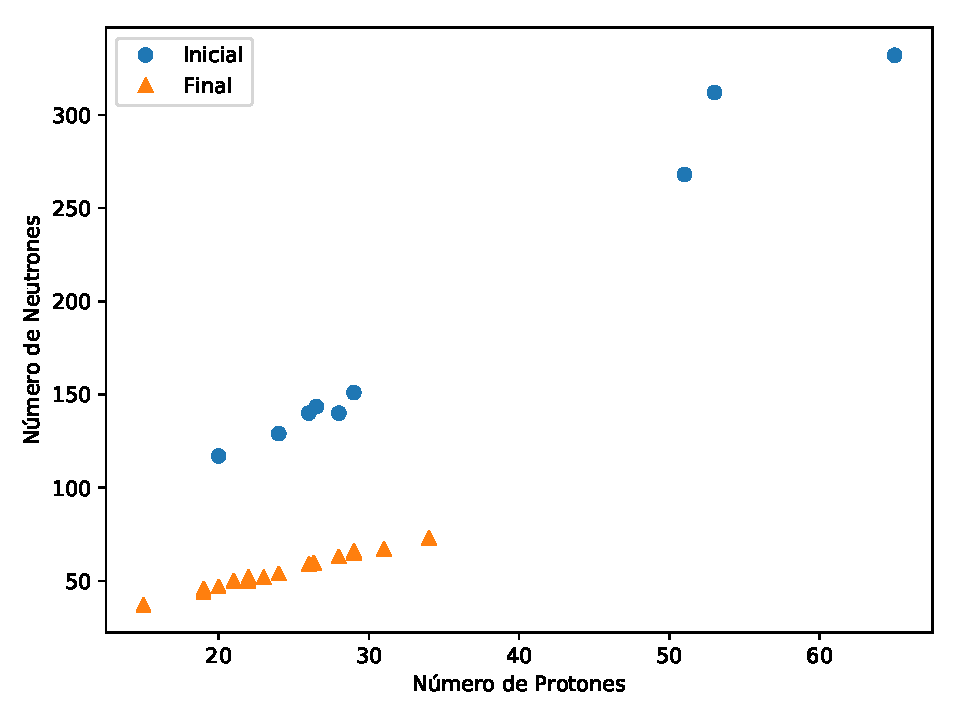
\includegraphics[width=0.8\columnwidth]{dinamica/mste}
  \caption{Distribución asintótica e inicial de masas para un sistema con $x = 0.1$, $\rho = 0.05\,\text{fm}^{-3}$ y $T = 0.1\,\text{MeV}$, para una expansión lenta ($\dot{\eta} = 0.0001\text{c/fm}$), con el algoritmo de reconocimiento MSTE.}
\label{fig:mste_pregnocchi}
\end{figure}

\begin{figure}
  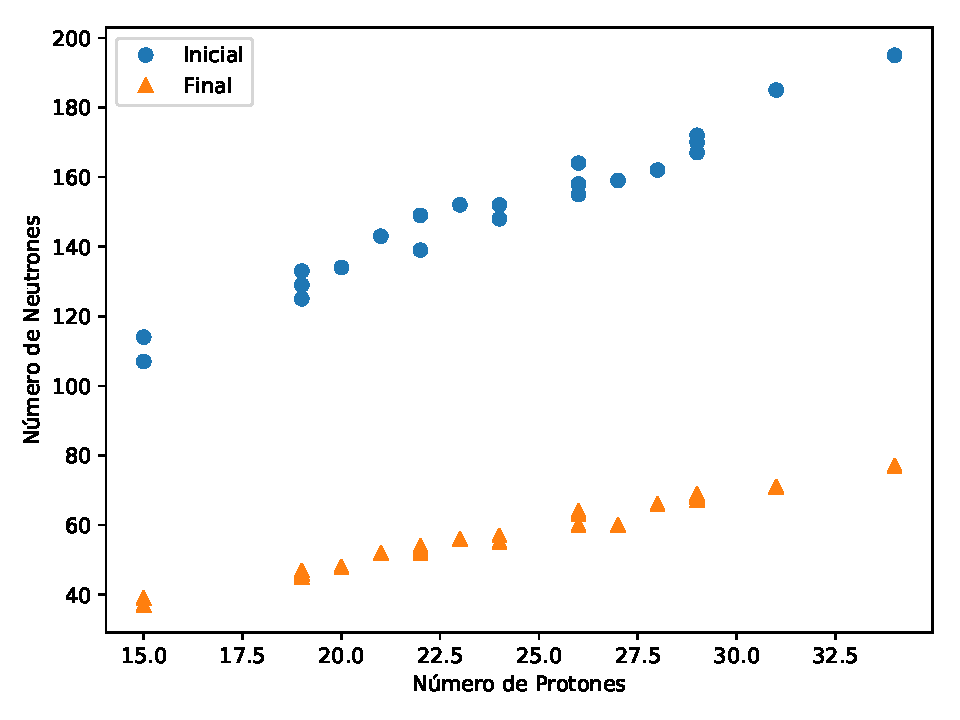
\includegraphics[width=0.8\columnwidth]{dinamica/mst_nube}
  \caption{Distribución asintótica e inicial de masas para un sistema con $x = 0.1$, $\rho = 0.05\,\text{fm}^{-3}$ y $T = 0.1\,\text{MeV}$, para una expansión lenta ($\dot{\eta} = 0.0001\text{c/fm}$), con el algoritmo de reconocimiento MST para protones.}
\label{fig:mst_pregnocchi}
\end{figure}

Para analizar esto, estudaimos la distribución con el algoritmo MST aplicado a los protones solos, mostrados en la figura~\ref{fig:mst_pregnocchi}.
De acuerdo a esta figura, vemos que la distribución de fragmentos ed los protones no cambió sustancialemte (sólo un cluster de protones se rompió) y, efectivamente, el fragmento más grande tiene 32 protones.
¿Qué tipo de resultados se obtienen del algoritmo ECRA, teóricamente más sólido?
En la figura~\ref{fig:ecra_pregnocchi} mostramos que de hecho el algoritmo ECRA-BFM dio buenos resultados, e identifica los preclusters adecuadamente, incluso encontrando el fragmento que se rompió.

\begin{figure}
  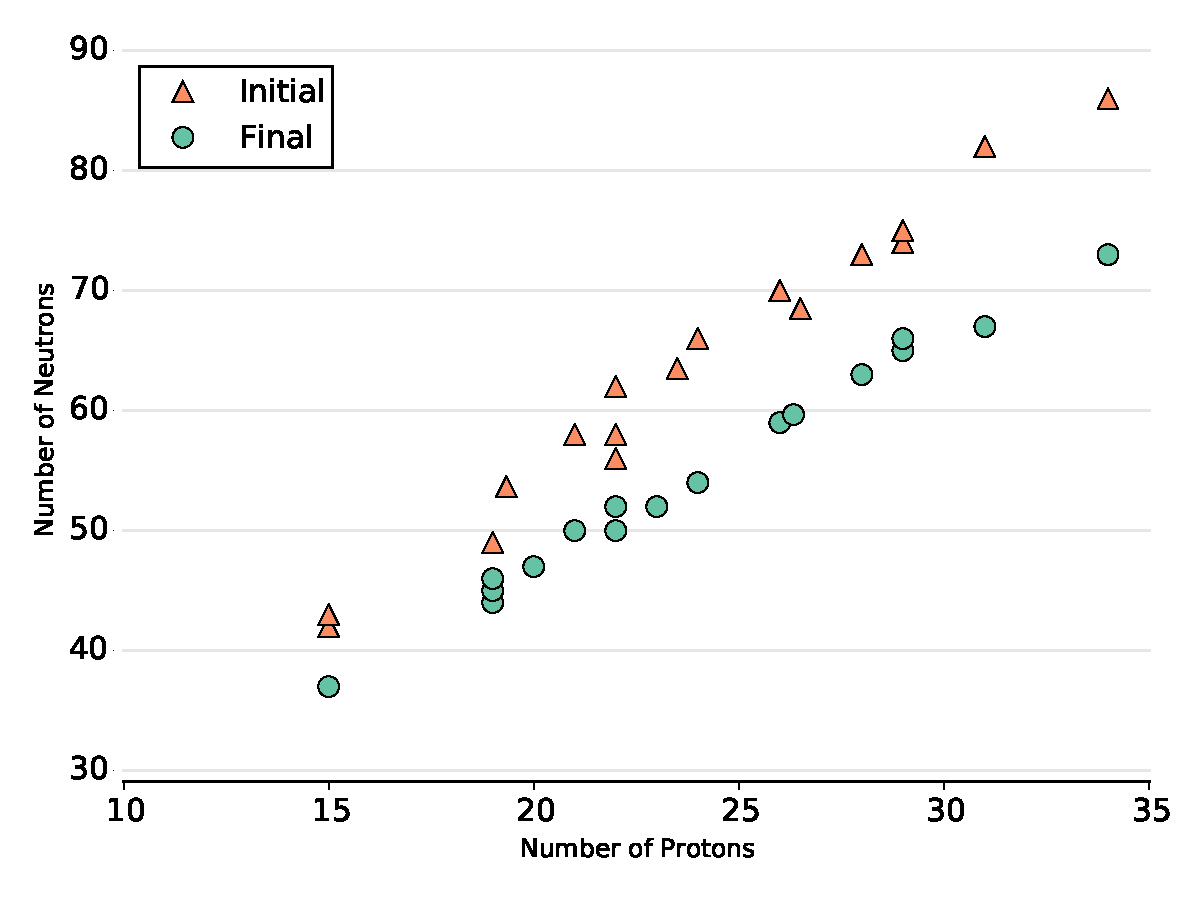
\includegraphics[width=0.8\columnwidth]{dinamica/ecra}
  \caption{Distribución asintótica e inicial de masas para un sistema con $x = 0.1$, $\rho = 0.05\,\text{fm}^{-3}$ y $T = 0.1\,\text{MeV}$, para una expansión lenta ($\dot{\eta} = 0.0001\text{c/fm}$), con el algoritmo de reconocimiento ECRA. Al comprarar con la figura~\ref{fig:mst_pregnocchi}, notar la diferencia de escalas en el eje $y$.}
\label{fig:ecra_pregnocchi}
\end{figure}

Con estos resultados en mente, utilizamos tres herramientas para el reconocimiento de fragmentos: MSTE, ECRA and MSTpC.
MSTE y ECRA son los algoritmos ya descritos, mientras que MSTEpC es el algoritmo de MST sobre protones con la nube de neutrones que están cerca de cada cluster MST.\@
En la figura~\ref{fig:lm_pre} mostramos la evolución del tamaño del fragmento más grande para las etapas iniciales de la evolución para los tres reconocedores de fragmentos: MSTE, MSTpC y ECRA.\@
La figura muestra que el fragmento ECRA se estabiliza rápido y se mantiene relativamente estable, mientras que los otros dos algoritmos resultan en fragmentos que son siempre más grandes que los ECRA y se estabilizan más lentamente.
También es interesante notar que el fragmento MSTpC comienza con alrededor de 100 neutrones más que el fragmento ECRA correspondiente, lo que implica que el fragmento de ECRA está en un ambiente muy rico en neutrones.
Esta situación hace que el \emph{r-process} sea más probable.

Por el otro lado, en la expansión de la estructura de \emph{lasagna}, ninguno de los algoritmos reconocedores de fragmentos identifican fragmentos en tiempos muy tempranos de la evolución (ver figura~\ref{fig:lm_las}).
En esta etapa hay un fragmento muy grande (que, de hecho, es infinito).
De cualquier modo, el análisis de ECRA muesra que este fragmento se parte tempranoamente en muchos fragmentos y, como resultado, la masas del fragmento más grande decrece drásticamente con el tiempo.
Es interesante notar que, a diferencia de los \emph{pregnocchi}, en este caso el algoritmo MSTpC es el que más tiempo toma para identificar que el fragmento infinito se parte.
Esto muestra que el algoritmo de ECRA es además más versátil para estudiar la formación temprana de fragmentos.
También es interesante notar (no se muestra en las figuras) que la fracción de protones $x$ de estos fragmentos es relativamente estable para el algoritmo ECRA, mientras que los otros dos resultan en una fracción de protones que decae monótonamente con el tiempo.

\begin{figure}[H]  \centering
  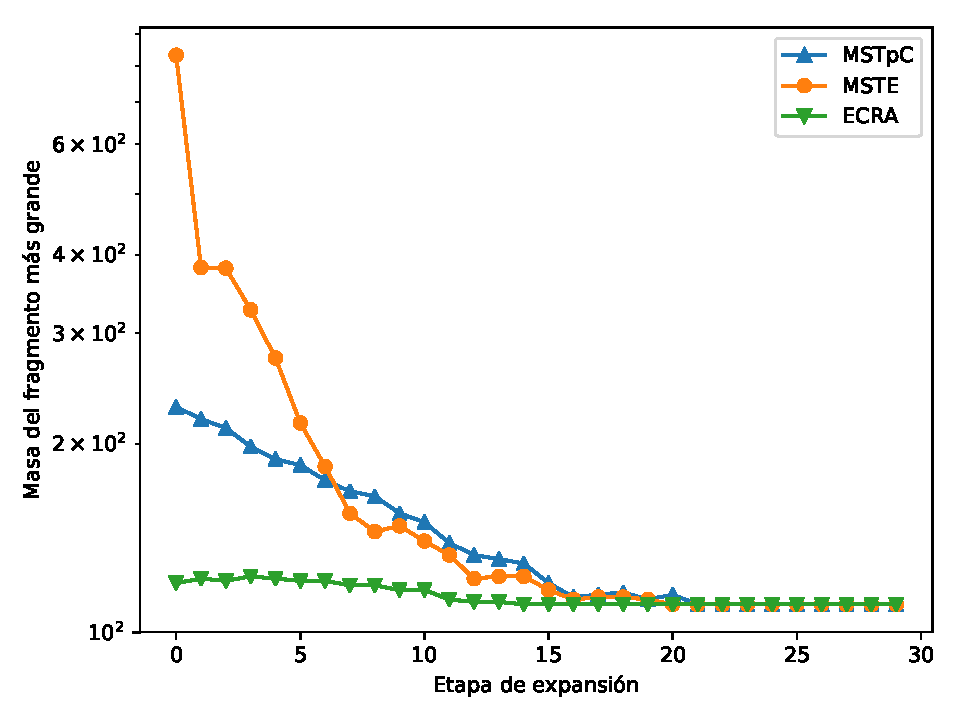
\includegraphics[width=0.8\columnwidth]{dinamica/lm_pre}
  \caption{Masa del fragmento más grande para MSTE, MSTpC y ECRA para las etapas iniciales de la evolución, para la configuración \emph{pre-gnocchi}.
    Se puede observar que el fragmento de ECRA se mantiene relativamente estable y se estabiliza rápidamente, mientras que los otros dos algoritmos ersultan en fragmentos que son siempre más grandes y tardan más en estabilizarse.}
\label{fig:lm_pre}
\end{figure}

\begin{figure}[H]  \centering
  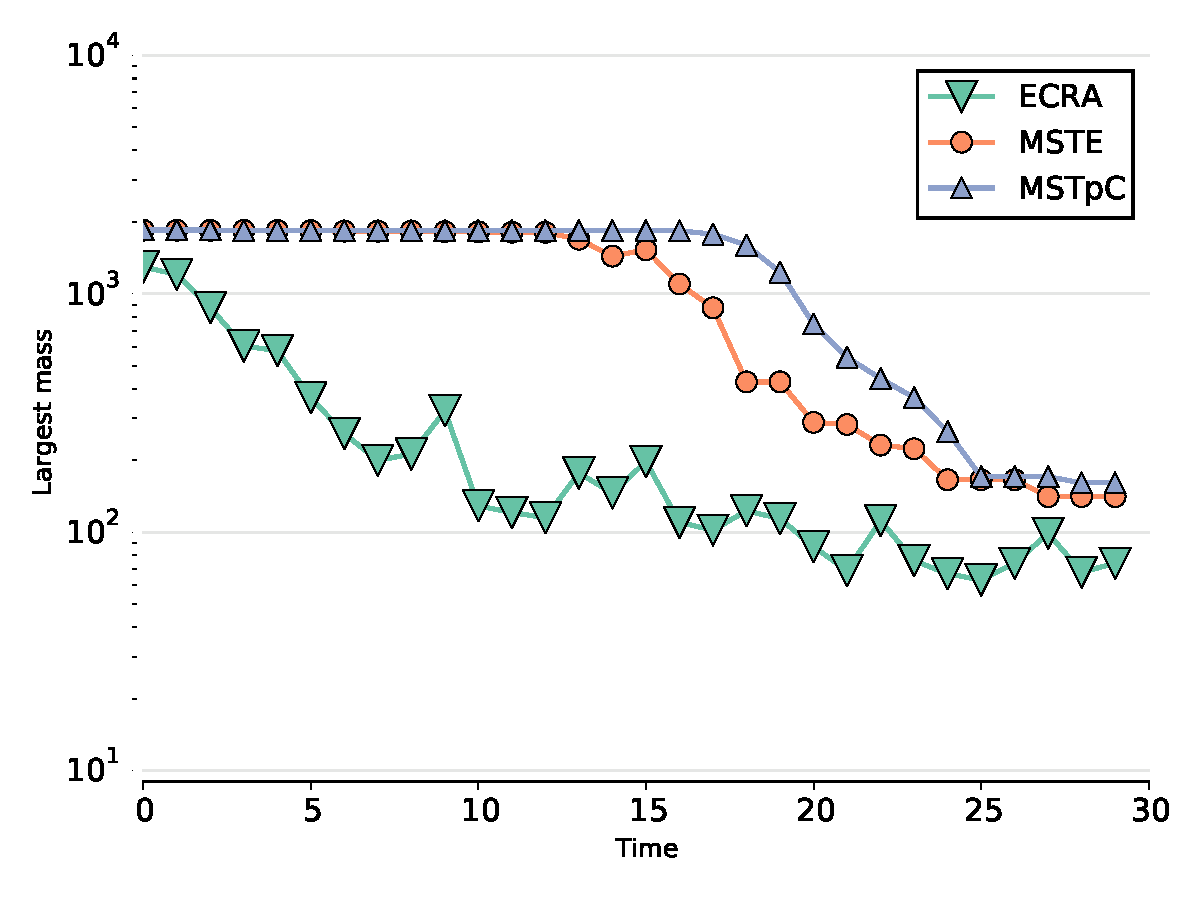
\includegraphics[width=0.8\columnwidth]{dinamica/lm_las}
  \caption{Masa del fragmento más grande para MSTE, MSTpC y ECRA para las etapas iniciales de la evolución, para la configuración \emph{lasagna}.
    Aquí se puede notar que, como en el caso anterior, el algoritmo ECRA reconoce la fractura del fragmento infinito muy tempranamente.
    En el régimen asintótico (por tiempos muy largos, no se muestra en las figuras) estos tres algoritmos dan los mismos resultados.}
\label{fig:lm_las}
\end{figure}


\section{Conclusiones}\label{sc:conc}

Estudiamos, con dinámica molecular, las propiedades estructurales de la corteza de estrellas de neutrones a través de tres potenciales distintos.
Estos potenciales involucran un término nuclear escogido para reproducir energías de ligadura y compresibilidad de la materia nuclear, sumado a la interacción de Coulomb.
Para analizar las estructuras que se forman utilizamos cuatro tipos distintos de algoritmos reconocedores de fragmentos: MST, MSTE, MSTpC y ECRA-BFM.
Con estos algoritmos encontramos que de los tres potenciales, dos de ellos (New Medium y SSP) desarrollaron una estructura nueva para bajas fracciones de protones que llamamos \emph{pregnocchi}.
Esta estructura consiste en agregados de protones formados por la mediación del término atractivo $V_{np}$ del potencial que resistieron la expansión.

También analizamos la expansión de materia rica en neutrones infinita descripta a través del modelo del pequeño big bang.
Mostramos que, en general, la identificación adecuada de la estructura depende mucho del algoritmo escogido, siendo ECRA y MSTpC los más adecuados para encontrar las estructuras y ECRA el más estable.
Este enfoque, combinado con distintos algoritmos reconocedores de fragmentos, nos perimitió identificar la dinámica de la formación de fragmentos.
El estado asintóticos mostró una alta dependencia con la velocidad de expansión, tanto en la distribución de masa como en la distribución espacial de los fragmentos: para velocidades suficientemente altas, la expansión era similar a una \emph{fractura mecánica}, donde la distribución espacial estaba altamente correlacionada con el estado original.
Sin embargo, para velocidades más bajas, la expansión era una \emph{expansión térmica}, en la que el estado asintótico era relativamente homogéneo.
Los fragmentos formados en la expansión más lenta eran mucho más grandes que los formados en la expansión rápida.
Un análisis cuidadoso de la dinámica de formación de fragmentos mostró que se formaron muy temprano en la expansión.
En particular, la novedosa estructura que llamamos \emph{pregnocchi} es de considerable relevancia, ya que de acuerdo al análsis de ECRA estos agregados preexistentes evolucionan en una nube de neutrones, resultando en configuraciones en las que el \emph{r-proccess} se puede desarrollar.

\section{Sobre la estabilidad de los clusters MSTE}
Un simple ejemplo puede ser estudiado para ver si los clusters MSTE son estables o no.
Consideremos una simple interacción del tipo pozo de potencial, en la que
\begin{equation}
V_{ij}(r) =
\begin{cases}
-V_0 &\text{if } r \leq a\\[2ex]
0 &\text{if } r > a.
\end{cases}
\end{equation}

Estudiemos ahora un conjunto de partículas de masa $m$ con posiciones $r_i = i\,a$ (con $i \in \mathcal{Z}$) tal que todas las partícuals están a distancia $a$ de sus vecinos más cercanos.
Si la velocidad es $v_i = i\,v$, cada parícula va a estar unida energéticamente con sus vecinos siempre que $v \leq \sqrt{2\,V_0/m}$.
Para $2n+1$ partículas, con $-n \leq i \leq n$, la energía cinética del sistema será
\begin{align}
  K_{\text{CM}} &= \sum_{i=-n}^n \frac{1}{2} m\, i^2 v^2\\
  &= \frac{n^3}{3}\,m\,v^2 + \mathcal{O}(n^2)
\end{align}

La energía potencial, sin embargo, es
\begin{align}
  V_{\text{CM}} &= \sum_{i=-n}^n -i V_0\\
  &= - 2\,n^2\,V_0
\end{align}

Es claro, entonces, que para $n$ grandes, sin importar el valor de $v$, el sistema es inestable más allá de que el algoritmo MSTE lo reconoce como un único cluster.
